\documentclass{article}

\usepackage[letterpaper, portrait, margin=1.5in]{geometry}

\usepackage{fancyhdr}
\usepackage{ragged2e}
\usepackage{graphicx}
\usepackage{caption}
\usepackage{amsmath}
\usepackage{rotating}

\usepackage{listings}
\usepackage{color}

\definecolor{dkgreen}{rgb}{0,0.6,0}
\definecolor{gray}{rgb}{0.5,0.5,0.5}
\definecolor{mauve}{rgb}{0.58,0,0.82}

\lstset{frame=tb,
  language=Java,
  aboveskip=3mm,
  belowskip=3mm,
  showstringspaces=false,
  columns=flexible,
  basicstyle={\small\ttfamily},
  numbers=none,
  numberstyle=\tiny\color{gray},
  keywordstyle=\color{blue},
  commentstyle=\color{dkgreen},
  stringstyle=\color{mauve},
  breaklines=true,
  breakatwhitespace=true,
  tabsize=4
}

\setcounter{secnumdepth}{1}

\usepackage{chngcntr}
\counterwithin{figure}{section}

\renewcommand*{\thepage}{C\arabic{page}}

\pagestyle{fancy}
\lhead{ACME Robotics}
\chead{\#8367}
\rhead{\ifcontents Contents \else Week \thesection \fi}

\newif\ifcontents
\contentstrue

\makeatletter
\renewcommand{\@seccntformat}[1]{}
\makeatother
\begin{document}

\subsection{Constructing the Pit}
%! things
With Worlds coming up quick, the team wanted to reconstruct and update their pit for Worlds. This included coming up with new swag and pit layout as well as putting the whole pit together to make sure they had all the pieces. ACME ended being very thankful they decided to this since they immediately ran into issues. As soon as they had gotten all the pieces of the pit ready to assemble, they realized no nobody remembered exactly how the pit was constructed. They had a basic idea of the structure, but not much beyond that. After much trial and error, diagram writing, organization, and pictures from last season, they finally figured how it all went together. To aid in construction and for future reference, the team made a diagram of what the pit should look like, as seen in Figure \ref{fig:diagram}. This whole process gave the team a lesson in documentation. If the team had just done some simple documentation when creating and constructing the pit last year, they could have avoided the issue entirely. This also made the team realize why its important to test and rehearse things. If the team hadn't checked to make sure everything was in order, they would have had some serious trouble at Worlds. Determined not make the same mistake twice, the team put Jon in charge of documentation and planning of the pit. To do this, Jon drew up a diagram of the pit with all the dimensions and the joint connector placements. This diagram was similar to the one made during reconstructing but with more detail and a simple top down view of the pit layout. As can be seen in Figure \ref{fig:pitone}. After constructing the pit itself, Jon, Aidan, and Ashlin, also labeled each part of the structure of the pit so it could hopefully be constructed without any diagrams. Finally Jon took pictures of the pit structure for redundancy. ACME hoped that this would be enough for anyone in future to construct the pit even without the help of someone who had done it before.

\begin{figure}
    \centering
    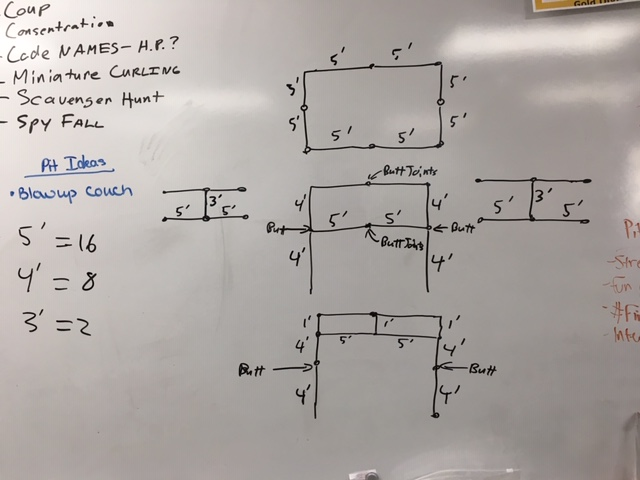
\includegraphics[width= 0.5 \textwidth]{30_03-25/images/pitdiagram1.JPG}
    \caption{Diagram of Pit parts}
    \label{fig:pitone}
\end{figure}

\begin{figure}
    \centering
    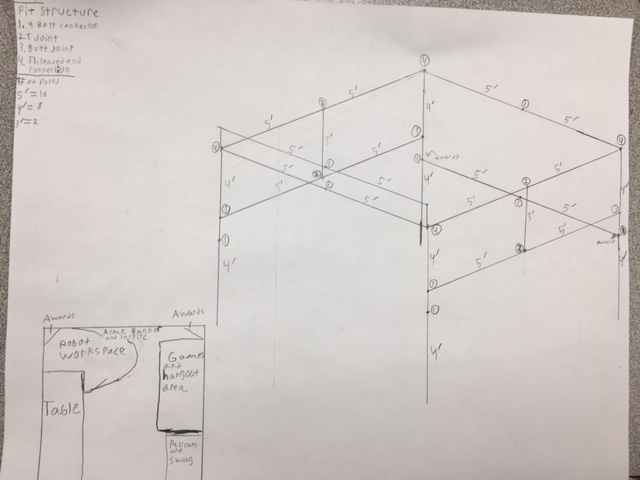
\includegraphics[width= 0.5 \textwidth]{30_03-25/images/pitdiagram2.JPG}
    \caption{Diagram of Pit dimensions and layout}
    \label{fig:finishedpit}
\end{figure}

\begin{figure}
    \centering
    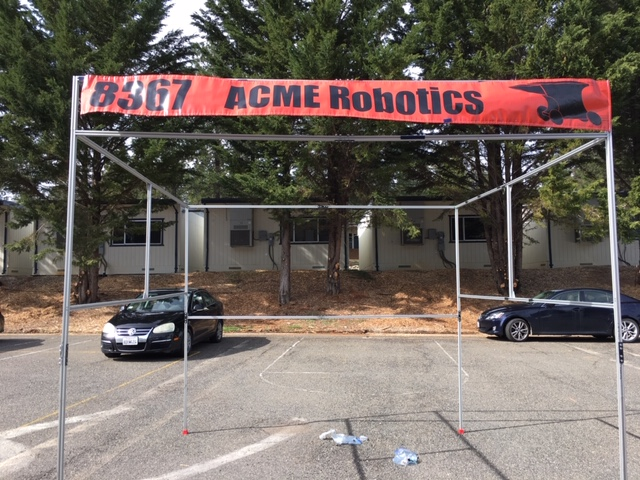
\includegraphics[width= 0.5 \textwidth]{30_03-25/images/pitpicture.JPG}
    \caption{Picture of pit for documentation}
    \label{fig:diagram}
\end{figure}

\subsection{Wiring}
%! things
Oren spent a lot of time directing the lift and rake wires that cross the drive-train to ensure that they didn't interfere with moving components and would be easy to swap out if necessary. This means that if in competition, it will be much easier to replace wires should the need arise. 


\end{document}